\documentclass[11pt, oneside]{article} 
\usepackage{geometry}
\geometry{letterpaper} 
\usepackage{graphicx}
	
\usepackage{amssymb}
\usepackage{amsmath}
\usepackage{parskip}
\usepackage{color}
\usepackage{hyperref}

\graphicspath{{/Users/telliott/Dropbox/Github-Math/figures/}}
% \begin{center} \includegraphics [scale=0.4] {gauss3.png} \end{center}

\title{Quadratics problems}
\date{}

\begin{document}
\maketitle
\Large

%[my-super-duper-separator]

\subsection*{Introductory examples}

A quadratic equation contains the square of a variable multiplied by some constant, which may be $1$.  Often we call the variables $y$ and $x$, so we have something like
\[ y = ax^2 \]

It may be that $a = 1$, and then $y = x^2$, but $a$ cannot be zero, or we don't have a quadratic.  

Then in addition there may be an optional term containing the first power of $x$ and also perhaps a final constant.  The general form is
\[ y = ax^2 + bx + c \]
where $a, b$ and $c$ are constants.  $b$ or $c$ (or both) might be zero.

The two most common applications are maximization problems, and gravity.

\subsection*{maximizing area}
We need to build a fence or a wall from a fixed amount of material.  There are constraints:   it must be in the shape of a rectangle, and we want the area enclosed to be a maximum.

You will usually be given some definite amount of material, like $100$ feet of fencing, but it does no harm to re-scale our problem, as long as we understand how to undo the scaling once we have the answer.

Let the perimeter of the rectangle be $2$, the half-perimeter is $1$, and then if one dimension, say the short side of the rectangle is $h$, the width is $1 - h$, so the area is
\[ A = hw = h(1 - h) = -h^2 + h \]

As will be obvious later, since $a < 0$, the graph of this equation forms a "cup" that opens down.  The value of $A$ at the vertex is a maximum.

Two fundamental facts about parabolas:   

$\circ$ \ the maximum (or minimum) always occurs at the vertex

$\circ$ \ the $x$-coordinate of the vertex has the value $-b/2a$

So the simplest parabola $y = x^2$ has $b = 0$, because there is no term like $bx$, and the vertex is at $x = 0$, $y = 0$.

In our problem $a = -1$ and $b = 1$, the vertex is the maximum and it is at $h = 1/2$.   Since $h + w = 1$, it follows that $h = w = 1/2$.

The meaning of this answer is that the square ($h = w$) has the maximum area for a rectangular shape with a fixed perimeter.

Actually, you may know that if the shape is not rectangular the maximum area is for a circle or disk, but that is not the problem we're solving!

\subsection*{gravity}

A second application is for objects falling under the influence of gravity.  Gravity is an acceleration, and that acceleration is constant, which means that if the speed or velocity after falling for one second is $v$, the velocity after two seconds is twice $v$ and so on.  

So the distance $d = vt$ covered from zero time up to 1 second is less than that covered between $t = 1$ and $t = 2$ seconds.  

Let me just give you the equation.  If we drop our rock from the Tower of Pisa and the tower stands a height $h_0$ above the ground, the distance $h$ above the ground after $t$ seconds is
\[ h = -16t^2 + h_0 \]
This makes sense.  At $t = 0$, $h = h_0$ and then $h$ will be smaller than $h_0$ by some amount $-16t^2$ when $t > 0$.

If the initial height $h_0$ is $144$ feet, then a dropped rock will hit the ground at $h=0$ which means that
\[ 0 = -16t^2 + 144 \]
\[ t = \sqrt{144/16} = \sqrt{9} = 3 \text{ sec} \]

We take only the positive square root, but to explain that will take more time than we want for this example right now.  We'll come back to it.

There is a limit to the final, or terminal velocity.  It comes not from gravity but from air resistance.  Someone who jumps from an airplane or gets thrown out through a window of the Nakatomi Plaza has a terminal velocity of about $180$ feet per second or $120$ miles per hour.

\subsection*{maximizing profit}
You are the producer of a Broadway show.  The theater seats 120 people and you have priced the tickets at \$10 each.  You always fill the theater.

It costs you \$200 to rent the theater and another \$200 to pay the cast, so the fixed costs $F$ are $400$ and your profit for each show is
\[ P = nT - F \]
\[ = 120 \cdot 10 - 400 = 800 \]

\$800 per show.  That seems pretty good.

Your cousin Vinnie has an idea:  if you raise the price you'll make more money.  However, you'll also sell fewer tickets.  Acme Consulting has done a study which says that for every \$1 increase in the ticket price you'll have two empty seats.

As a red-blooded American, \emph{of course} you want the maximum profit.  What should you do?  There's clearly money to be made, if you raise the ticket price \$1, you'll sell 118 seats at \$11 for \$1298, giving a net profit of \$898.

Call the price increase $x$.  You will sell $n - 2x$ seats at a ticket price of $T + x$ for a profit
\[ P = (n - 2x)(T + x) - 400 \]
\[ = -2x^2 + (n - 2T)x + nT - 400 \]

The $x$ corresponding to the maximum of this quadratic is $-b/2a$.

\[ x  = -(n - 2T)/2(-2) \]
\[   = (120 - 20)/4 = 25 \]

You increase the ticket price from \$10 to \$35.  The profit will be
\[ P = (n - 50)(T + 25) - 400 \]
\[ = 70 \cdot 35 - 400 = 2050 \]
That's an increase of \$1250 per show.

\subsection*{sum and product}

The sum of two numbers is 18 and their product is 56.  What are they?

\[ u + v = 18 \]
\[ uv = 56 \]

\[ u(18 - u) = 56 \]
\[ u^2 - 18u + 56 = 0 \]

The factors of $56$ are $2 \cdot 28$, $4 \cdot 14$, and $7 \cdot 8$.
\[ 4 + 14 = 18 \]
so
\[ (u - 4)(u - 14) = 0 \]

The numbers are $4$ and $14$.

\subsection*{odd numbers}
The product of two consecutive positive odd numbers is $255$.  Find the numbers.

Odd numbers can be described as $2n+1$ for some $n$, since that is one more than the even number $2n$.  So we have
\[ (2n + 1)(2n + 3) = 255 \]
\[ 4n^2 + 8n + 3 = 255 \]
\[ 4n^2 + 8n - 252 = 0 \]
We are looking for zeros.  So we can divide by $4$:
\[ n^2 + 2n - 63 = 0 \]
Two numbers multiply to give $-63$ and add to give $2$:
\[ (n + 9)(n - 7) = 0 \]
The roots are $-9, 7$.  But we specified positive numbers which means $n = 7$.  The numbers are $2 \cdot 7 + 1 = 15$ and $17$, easily confirmed.

Alternatively we can write the numbers as $2n + 1$ and $2n - 1$ and then
\[ (2n + 1)(2n - 1) = 255 \]
\[ 4n^2 - 1 = 255 \]
\[ n^2 = 64 \]
\[ n = \pm 8 \]
Again $n > 0$ so $n = 8$ and the numbers are $2n - 1 = 15$ and $2n + 1 = 17$.

\subsection*{bus trip}

By going $15$ km per hr faster, a transit bus would have required 1 hr less to travel $180$ km. What was the average speed of this bus?

Velocity $\times$ time = distance.

\[ vt = 180 \]
\[ (v + 15)(t - 1) = 180 \]

We can eliminate either $v$ or $t$.  Let's try $v$ first.

\[ v = 180/t \]
\[ v + 15 = 180/(t-1) \]
\[ 15 = 180/(t-1) - 180/t \]

\[ 15(t^2 - t) = 180t - 180(t-1) \]
\[ 15(t^2 - t) - 180 = 0 \]
\[ t^2 - t - 12 = 0 \]
\[ (t + 3)(t - 4) = 0 \]
\[ t = -3,4 \]

We choose $t = 4$ so then $v = 45$ and $180/60 = 3$ checks.
The answer is $v = 45$.

\subsection*{area of a square}

If the length of each side of a square is increased by 6, the area is multiplied by 16. Find the side length of the original square.

Let the original side be $x$ and the original area is $x^2$, so the new area is 

\[ 16x^2 = (x + 6)^2 \]
 \[      = x^2 + 12x + 36 \]
then
\[ 15x^2 - 12x - 36 = 0 \]

Factor out $3$
\[ 5x^2 - 4x - 12 = 0 \]
\[ (5x + \text{ ?})(x + \text{ ?}) = 0 \]
Go through the factors of $12$ to find $2$ and $6$ and then $5 \cdot 2 - 6$ gives $4$ so
\[ (5x + 6)(x - 2) = 0 \]

Lengths are positive, so $x = 2$.
\[ 2^2 \cdot 16 = 64 = (2 + 6)^2  \]

\subsection*{swimming pool}

You live in a fancy suburban neighborhood where all the houses have pools.  It's very cold in winter where you live, and all the pools are drained so they won't crack.

Suppose your garden hose can fill your swimming pool in $x$ days.  Your neighbor has a pool the same size as yours, but a bigger hose, so she can fill her pool in $y$ days.  Suppose you know that $y + 6 = x$.  

Last year, you both started on the same day, but then you forgot what date that was, all you know is that she finished 6 days before you.

The next year when you need to refill your pool, you put both hoses together, to fill your pool in $z$ days.

The rates are what add, and rates are amount divided by time.  If the volume of the pool is $V$ then
\[ \frac{V}{x} + \frac{V}{y} = \frac{V}{z} \]
\[ \frac{1}{x} + \frac{1}{y} = \frac{1}{z} \]
\[ yz + xz = xy \]

As we said, $y + 6 = x$.  When you use both hoses together, it takes only 4 days to fill your pool.  How long would it take if you used only your own hose?  What is $x$?

We have that $z = 4$.
\[ 4y + 4x = xy \]
And then $y = x - 6$ so
\[ 4(x - 6) + 4x = x(x - 6) \]
\[ 8x - 24 = x^2 - 6x \]
\[ x^2 - 14x + 24 = 0 \]
\[ (x - 2)(x - 12) = 0 \]

There are two roots, but $x = 2$ leads to the non-sensical answer that $y = -4$.  So we will settle on $x = 12$, then $y = 6$.  We know $z = 4$ and indeed
\[ \frac{1}{12} + \frac{1}{6} = \frac{1}{4} \]
or if you prefer
\[ 6 \cdot 4 + 12 \cdot 4 = 6 \cdot 12 \]

\subsection*{electricity}
Here's a problem involving electricity but we will tell you the analysis so you don't need to known any physics.  In fact, you could just skip ahead to the equation.

The current $I$ that flows along a wire is equal to the difference in voltage $V$ across the two ends, divided by the resistance $R$.
\[ I = \frac{V}{R} \ \ \ \ \ \ \ \ V = IR \]

Imagine that the wire itself has negligible resistance, but there are two things called resistors $R$ hooked up in an arrangement called \emph{parallel}.  If you connect a battery (voltage $V$) to the two wires on the ends of this circuit
%\begin{center} \includegraphics [scale=0.6] {resistors.png} \end{center}
there will be some total current ($I_T$) that flows.  Those electrons go either one way or the other across the two resistors.  So the current is what adds
\[ I_T = I_1 + I_2 \]
\[ \frac{V}{R_T} = \frac{V}{R_1} + \frac{V}{R_2} \]

Which is a long-winded way of saying that the reciprocal of the resistance adds.
\[ \frac{1}{R_T} = \frac{1}{R_1} + \frac{1}{R_2} \]

Suppose we're given that $R_2 = R_1 + 3$ and that $R_T = 2$.  I want to use $r$ for $R_1$.  We have
\[ \frac{1}{r} + \frac{1}{r+3} = \frac{1}{2} \]
Naturally we want to find $r$.  Multiply out
\[ (r + r + 3)(2) = r(r + 3) \]
\[ r^2 -r - 6 = 0 \]
\[ (r-3)(r+2) = 0 \]
So $r = 3, -2$.  We choose $r = 3$ and then $R1 = 3$, $R2 = 6$ and
\[ 1/3 + 1/6 = 3/6 = 1/2 \]
Checks.

\subsection*{river travel}

You travel from home to market on a river that flows at 2 km/hr.  Your motorboat goes at a constant speed, and the distance to market downriver is 12 km.

Then you drop off your bananas, and immediately turn around and come back home.  The total travel time is 8 hr.  

How fast does the boat go in still water?

\emph{Solution}.

Let $v$ be the velocity of the boat.  On the trip downriver the speed (with respect to the shore) is $v + 2$, while coming home it is $v - 2$.  Let $t$ be the time going to market and $t'$ be the time coming home.

Velocity $\times$ time equals distance.  We can write two equations:

\[ 12 = (v + 2) t \]
\[ 12 = (v - 2) t' \]

Plus we have
\[ t + t' = 8 \]

We can eliminate $t$ by isolating it in the first two equations and then adding.

\[ \frac{12}{v+2} + \frac{12}{v-2}= t + t' = 8 \]

Now it's just rearranging
\[ 12(v - 2 + v + 2) = 8(v - 2)(v + 2) \]
\[ 12(2v) = 8(v - 2)(v + 2) \]
We have a quadratic:
\[ 3v = v^2 - 4 \]
\[ v^2 - 3v - 4 = 0 \]
\[ (v - 4)(v + 1) = 0 \]

Factoring works for this example.  

The velocity must be positive, and of the two roots, only one is positive.  

$v = 4$ so the velocity downriver is $6$ km/hr and upriver it is $2$ km/hr.  The trip downriver takes 2 hr and upriver it takes 6 hr for a total of 8 hr.

Here is another approach.  Substitute for $t'$ right away.
\[ 12 = (v + 2) t \]
\[ 12 = (v - 2) (8 - t) \]
Multiplying out
\[ 12 = vt + 2t \]
\[ 12 = 8v - vt - 16 + 2t \]

Add to get rid of $vt$
\[ 24 = 8v - 16 + 4t \]
Factor out a $4$
\[ 6 = 2v - 4 + t \]
Above, we have $t = 12/(v+2)$ so
\[ 6(v+2) = (v+2)(2v-4) + 12 \]
\[ 6v + 12 = 2v^2 - 8 + 12 \]
Factor out $2$
\[ 3v + 6 = v^2 - 4 + 6 \]
\[ v^2 - 3v - 4 = 0 \]
\[ (v - 4)(v + 1) = 0 \]
We obtain the same result.

Graphing often adds insight:
%\begin{center} \includegraphics [scale=0.5] {river_hyper.png} \end{center}

\subsection*{gravity}
Many problems for quadratics involve gravity because the distance an object falls under gravity goes like $t^2$.  That was Galileo's famous discovery.  He used an inclined ramp and a water clock.  

The business about dropping objects of different weights off the Tower of Pisa was a popular activity during the century preceding Galileo.  His contribution was a thought experiment that is even more interesting.

\url{https://en.wikipedia.org/wiki/Galileo%27s_Leaning_Tower_of_Pisa_experiment}

In the metric system, the acceleration due to gravity (near the earth's surface) is very close to $10$ meters per second$^2$.  So, if we drop a rock, the distance traveled goes like 
\[ d = \frac{1}{2} 10 \ t^2 = 5 \ t^2 \]
After $1$ second, $5$ meters, after $2$ seconds $20$ meters, and so on.  If we know the distance to the ground and want the time:
\[ t = \sqrt{\frac{d}{5}} \]

Some problems involve throwing an object up in the air to begin with, then we need the general equation for movement in one dimension.
\[ x = \frac{1}{2}at^2 + v_0 t + x_0 \]

Which letter to use for the variable is your decision and really makes no difference.  We can use $y$ for height, by analogy with our graphs on the $xy$-axes.  We can use $h$, for height, or $d$ for distance.  Or we can just use $x$, as we might in outer space.

$x$ is really $x(t)$, the $x$-position depends on, it is \emph{a function of}, the time.  

The distance depends on the initial velocity $v_0$ times the time, which makes sense, and on the initial position $x_0$.

To use this equation we must keep our directions straight.  Gravity accelerates downward, normally initial heights will be positive, and initial velocity is usually positive but may be negative.  And of course the velocity may start positive but then surely turns negative, because gravity always wins.

You might be wondering about the other term, so consider a situation where $v_0$ and $x_0$ are both zero.  Then
\[ x = \frac{1}{2}at^2 \]

There's a bit of a mystery here, why do we have the factor of $1/2$, given the $v = at$?  

The $v$ in this formula is the velocity at the end of the interval, after $a$ has acted to boost the velocity from $v_0$ to $v$.

The correct relationship \emph{really} is
\[ x = \bar{v} t \]
where $\bar{v}$ is the average velocity
\[ \bar{v} = \frac{1}{2}at \]

We explore this a bit more in the next section.

\subsection*{time-dependence}
Distance equals velocity times time.

This is easy if the velocity is constant.  Travel west on the interstate at exactly $60$ miles per hour for $2$ hours and your distance will be $120$ miles from where you started (provided you don't start in Los Angeles).  

It is standard to use $s$ to refer to the distance traveled and $v$ for velocity.  If the velocity is constant then:
\[ s = vt \]
According to the internet, $s$ is from the Latin "spatium", for "space, room, or distance."

Suppose we plot velocity as a \emph{function of time} with $v$ on the $y$-axis and $t$ on the $x$-axis.

%\begin{center} \includegraphics [scale=0.35] {velocity_time_3.png} \end{center}

Since the velocity is constant, the result is a straight horizontal line.  

Furthermore, the distance traveled is the \emph{area under the curve} (and above the $x$-axis) which is the area of a rectangle with sides $v$ and $t$ and as we said 
\[ s = vt \]

However, for most interesting problems the velocity is not constant.  

Imagine maintaining pressure on the gas pedal in the car steadily so that, starting from a stop at zero time, after $1$ second your velocity is $10$ mph, after $2$ seconds it is $20$ mph, after $3$ seconds, $30$ mph. If we continue at the same rate of acceleration, we'll go from $0$ to $60$ mph in $6$ seconds, which is quite a respectable time.

This example has constant acceleration.  Here, we say that $v$ is a constant function of time, and write 
\[ v = at \]
where $a$ is the acceleration.  It is the slope of the line.

%\begin{center} \includegraphics [scale=0.35] {velocity_time_4.png} \end{center}
What about the distance?  It turns out that the distance is once again the area under the curve.

If $a$ is non-zero and constant, then $v$ changes at a constant rate.  Starting from $0$, the final velocity will be $v = at$, but the distance traveled is no longer the product 
\[ s = v \times t \stackrel{?}{=}  \]

because this $v$ is the final velocity and that is not the correct $v$ to use.  For variable velocity, the distance traveled is the \emph{average} velocity times the time.  For smooth (constant) acceleration from zero to $v$, the average velocity is the average of the initial and final velocities:
\[ v_{\text{avg}} = \frac{1}{2} \ (v_i + v_f) = \frac{1}{2} \ v \]

So the correct equation is:
\[ s = v_{\text{avg}}\ t  = \frac{1}{2} \ v \cdot t \]
and since $v = at$
\[ s = \frac{1}{2} at^2 \]

In this case, if we plot velocity as a function of time, we obtain a straight line that extends diagonally up with respect to the $x$-axis.  The distance traveled is the area under the curve, below the line and above the $x$-axis.  

The shape whose area is needed is a triangle.  This also accounts for the factor of $1/2$.

$\bar{v}$ is the average velocity during the interval between $0$ and $t$.  Since the acceleration $a$ is a constant, this is simply the average of the velocity at the end $(v = at)$, and at the start $(v = 0)$.
\[ \bar{v} = \frac{1}{2} (v_f + v_0) = \frac{1}{2} (at + 0) = \frac{1}{2} at \]
So that's why there is a factor of one-half in the basic formula.
\[ x = \frac{1}{2}at^2 + v_0 t + x_0 \]

\subsection*{gravity}

The equation for gravity is
\[ h = \frac{1}{2}g t^2 + v_0 t + h_0 \]

This says that if we throw an object like a rock or a cannonball straight up into the air, the height at time $t$ depends on the acceleration due to gravity $g$, the initial velocity $v_0$ in the upward direction, and the initial height $h_0$ relative to the earth's surface.

For gravity we have only two directions in one dimension, up and down.  The constant $g$ is negative while $v_0$ and $h$ are positive, because the force of gravity points down while we have defined up as positive.  We can rewrite this as
\[ h = -16t^2 + vt + h_0 \]

Here the units of velocity $v$ are feet per second, $h$ is in feet, and $g$ is $-32$ feet per second per second.  (If this were a physics book we'd use meters, and then $g$ would be $-10 \ m/s^2$.

Suppose the initial height is $h_0 = 96$, which means that you are almost $100$ feet in the air, perhaps on a platform or the top of a cliff, and the initial velocity is upward at $32$ feet per second.  That's about 25 miles per hour.

Clearly the rock will go up to some maximum height and then come down.  The question asks first, at what time is the height a maximum?  Recall the formula for the vertex.
\[ m = -\frac{b}{2a} = -\frac{v_0}{2(-16)} = \frac{32}{32} = 1 \]

The rock reaches its maximum height at $1$ second and that height is
\[ h = -16(1)^2 + 32(1) + 96 = 112 \]

My little brother throws 25 miles per hour.  Suppose you could talk a professional baseball player into climbing up there with you and throwing vertically up at 64 feet per second.  A fun fact is that $15$ mph is exactly $22$ feet per second.
\[ 64 \ \frac{22}{15} \approx 95 \]
about 95 miles per hour, a fastball.

Then
\[ m = - \frac{v_0}{2(-16)} = \frac{-64}{-32} = 2 \]
Two seconds to the maximum height.

If he throws the rock straight up, it will land on his head, or yours, in a stiff breeze.  Suppose the player throws it outward a bit, but still up with the same velocity, so when it comes down it just misses his nose.  

At what time will it reach the ground?  We have
\[ h = 0 = -16t^2 + 64t + 96 \]
and we need the roots of this quadratic equation because we are asking for $h = 0$ which is ground level.

Do you remember where we said that the roots don't change if we factor out a constant?
\[ h = 0 = (-16)(t^2 - 4t - 6) \]

We can't factor this one into integers.  The times where $h = 0$ are, with $m = 2$ and $c = -6$:
\[ m \pm \ \sqrt{m^2 - c} = 2 \pm \ \sqrt{4 + 6} = 2 \pm \ 3.16 = - 1.16, 5.16 \]

This says that the rock hits the ground after 5 seconds or so.  

The negative root also can have a physical meaning under some conditions.  The equation doesn't know about the baseball player or the ladder.  All it knows is that we started our clock at zero with the rock at $96$ feet above the ground and a vertical velocity of $16$ feet per second upward.  We won't worry about that.

If we are not allowed to use the simplification gained by factoring $a$ and also told to use the quadratic equation, you will write
\[ -16t^2 + 64t + 96 = 0 \]

so
\[ x = \frac{-b \pm \ \sqrt{b^2 - 4ac}}{2a} \]
\[ x = \frac{-64 \pm \ \sqrt{64^2 -4(-16)(96)}}{2(-16)} \]

I get $10240$ for the discriminant and about $3.16$ for the square root after dividing by $32$.  That matches the previous answer.

We can also say something about the velocity.  The equation for velocity is
\[ v = gt + v_0 \]

The velocity at any time $t$ is equal to the initial value plus the change due to gravity.  Again, $g$ is negative while $v_0$ is positive.  Depending on time $t$, $v$ may be either positive or negative.  We had a factor of $1/2$ before, that is $(1/2)g = -16$, but $g = -32$.

There is one moment when the velocity is zero, when the height is a maximum and the rock stops going up and comes back down.

In this problem
\[ v = 0 = -32t + 64 \]
Again, $2$ seconds to maximum height.

At $t = 5.16$ the velocity is about
\[ v = -32 (5.16) + 64 = 100 \]

\subsection*{maximizing distance}
King Charles requires you to shoot a cannonball as far as possible.  The distance depends on the angle at which the projectile is fired (we ignore air resistance).  

This classic problem is usually solved by trigonometry, but we are going to do it directly.  The velocity is some combination of horizontal and vertical components $v_x$ and $v_y$

Using the Pythagorean theorem we have that
\[ v^2 = v_x^2 + v_y^2 \]

Aside from this relationship, the two component velocities act independently.  If not for gravity the horizontal distance $d$ would be 
\[ d = v_x t \]

and the clock would just keep ticking, so $d$ would continue to increase, as it would if the cannon were fired in outer space.

However, the clock must stop, because for reasonable values of the velocity, gravity will bring the cannonball back down to earth before it leaves the atmosphere.  That equation is
\[ y = -16t^2 + v_y t + 0 \]
We want the time when $y = 0$ so
\[ 16t^2 = v_y t \]

Since there are only two terms in this quadratic and they both contain $t$, we can simplify it by dividing out
\[ 16t = v_y \]
\[ t = \frac{v_y}{16} \]

Dividing both sides by $t$ in this way, we "lose" a solution, but that solution is $t = 0$, which we don't care about.  Now plug that expression for $t$ back into the first equation.
\[ d = \frac{v_x v_y}{16} \]

We need to choose $v_x$ and $v_y$ to maximize $d$.  We can ignore the factor of $1/16$, since the value of $v_x$ or $v_y$ giving a maximum for $d$ will also maximize $16d$.

In the end, we want to maximize
\[ v_x v_y = v_x \sqrt{v^2 - v_x^2} \]
where $v$ is a constant for a given cannon and amount of gunpowder, etc.

Just to explore a little, scale the problem so that $v = 1$, and come up with a simpler name for the variable $v_x$, like $s$.  Then take a look in Desmos
%\begin{center} \includegraphics [scale=0.5] {quad4.png} \end{center}

The curve doesn't look like a standard parabola (it actually is one, but rotated by an angle).  It seems that the maximum comes at roughly $s = 0.7$.  That's a hint, because we know that $1/\sqrt{2} \approx 0.7$.

Without getting into the gory details, there is no reason to favor $x$ over $y$.  We expect they should be equal.
\[ v^2 = v_x^2 + v_y^2 = 2 v_x^2 \]
\[ v_x = \frac{v}{\sqrt{2}} \]

The maximum comes when $v_x = v_y$, that is, for an angle of $45^{\circ}$.  I'm told this isn't true in real life, because of air resistance.

Putting this another way, to maximize this:
\[ v_x \sqrt{v^2 - v_x^2} \]
we maximize the square:
\[ v_x^2 (v^2 - v_x^2) \]

$v_x^2$ will be some fraction $f$ of $v^2$.
\[ fv^2 (v^2 - fv^2) = v^2 \ [ \ f(1-f) \ ] \]
$v$ is a non-zero constant, so this problem really amounts to maximizing $f (1-f)$.  The quadratic is 
\[ -f^2 + f = 0 \]
The maximum is $m = -b/2a = - (1)/(2)(-1) = 1/2$.  Plug it into Desmos and take a look.

So $v_x^2$ is one-half of $v^2$ and equal to $v_y^2$.  Hence $v_x = v_y$.

\subsection*{inclined plane}

Think about a ramp or inclined plane at some angle $\theta$ to the vertical.  Place a block of lead on the ramp and it slides down to the bottom.  We ignore friction.  

The vertical height is $h$, and the length of the ramp is $L$.  It always helps to draw a picture.
%\begin{center} \includegraphics [scale=0.4] {incline.png} \end{center}

It is a remarkable fact that forces (and most everything) can be converted easily between different coordinate systems.  

The force along the ramp, making the block move, is the component of gravity acting in that direction.  Using similar right triangles, it is easy to show that 
\[ \frac{h}{L} = \frac{g'}{g} \]
This is called the cosine of the angle $\theta$ but we don't need trigonometry for this problem.  

The point is that a part of the force of gravity still acts along an inclined plane, multiplied by a factor less than one and equal to $h/L$.  So our equation of motion is
\[ s = \frac{1}{2} g' t^2 + v_0 t + s_0 \]
where $g' = gh/L$.

When does the block reach the bottom?  Then, $s = L$ and
\[ L = \frac{1}{2} g' t^2 = 16 h/L \cdot t^2 \]
\[ t = \frac{L}{4 \sqrt{h}} \]

The velocity at the bottom is 
\[ v = g't = g h/L \cdot  \frac{L}{4 \sqrt{h}} = 8 \sqrt{h} \]
Perhaps surprisingly, the answer is independent of $L$.

Different ramp lengths give the same final velocity, though not the same time.

If you know simple physics we can do this problem in another way, namely by conservation of energy.
\[ P.E. = K.E. \]
The potential energy at the top is equal to the kinetic energy at the bottom.
\[ mgh = \frac{1}{2} mv^2 \]
\[ v^2 = 2gh = 64 h \]
\[ v =  8 \sqrt{h} \]
which is what we had before.

\subsection*{incircle and smaller circles}

Acheson presents this problem (though he does not show the solution).  The algebra defeated me for quite a long time, but I finally got it.

We are given only the radii of the small circles, $a,b$ and $c$, and are asked to find $r$, which I have written as $R$.

%\begin{center} 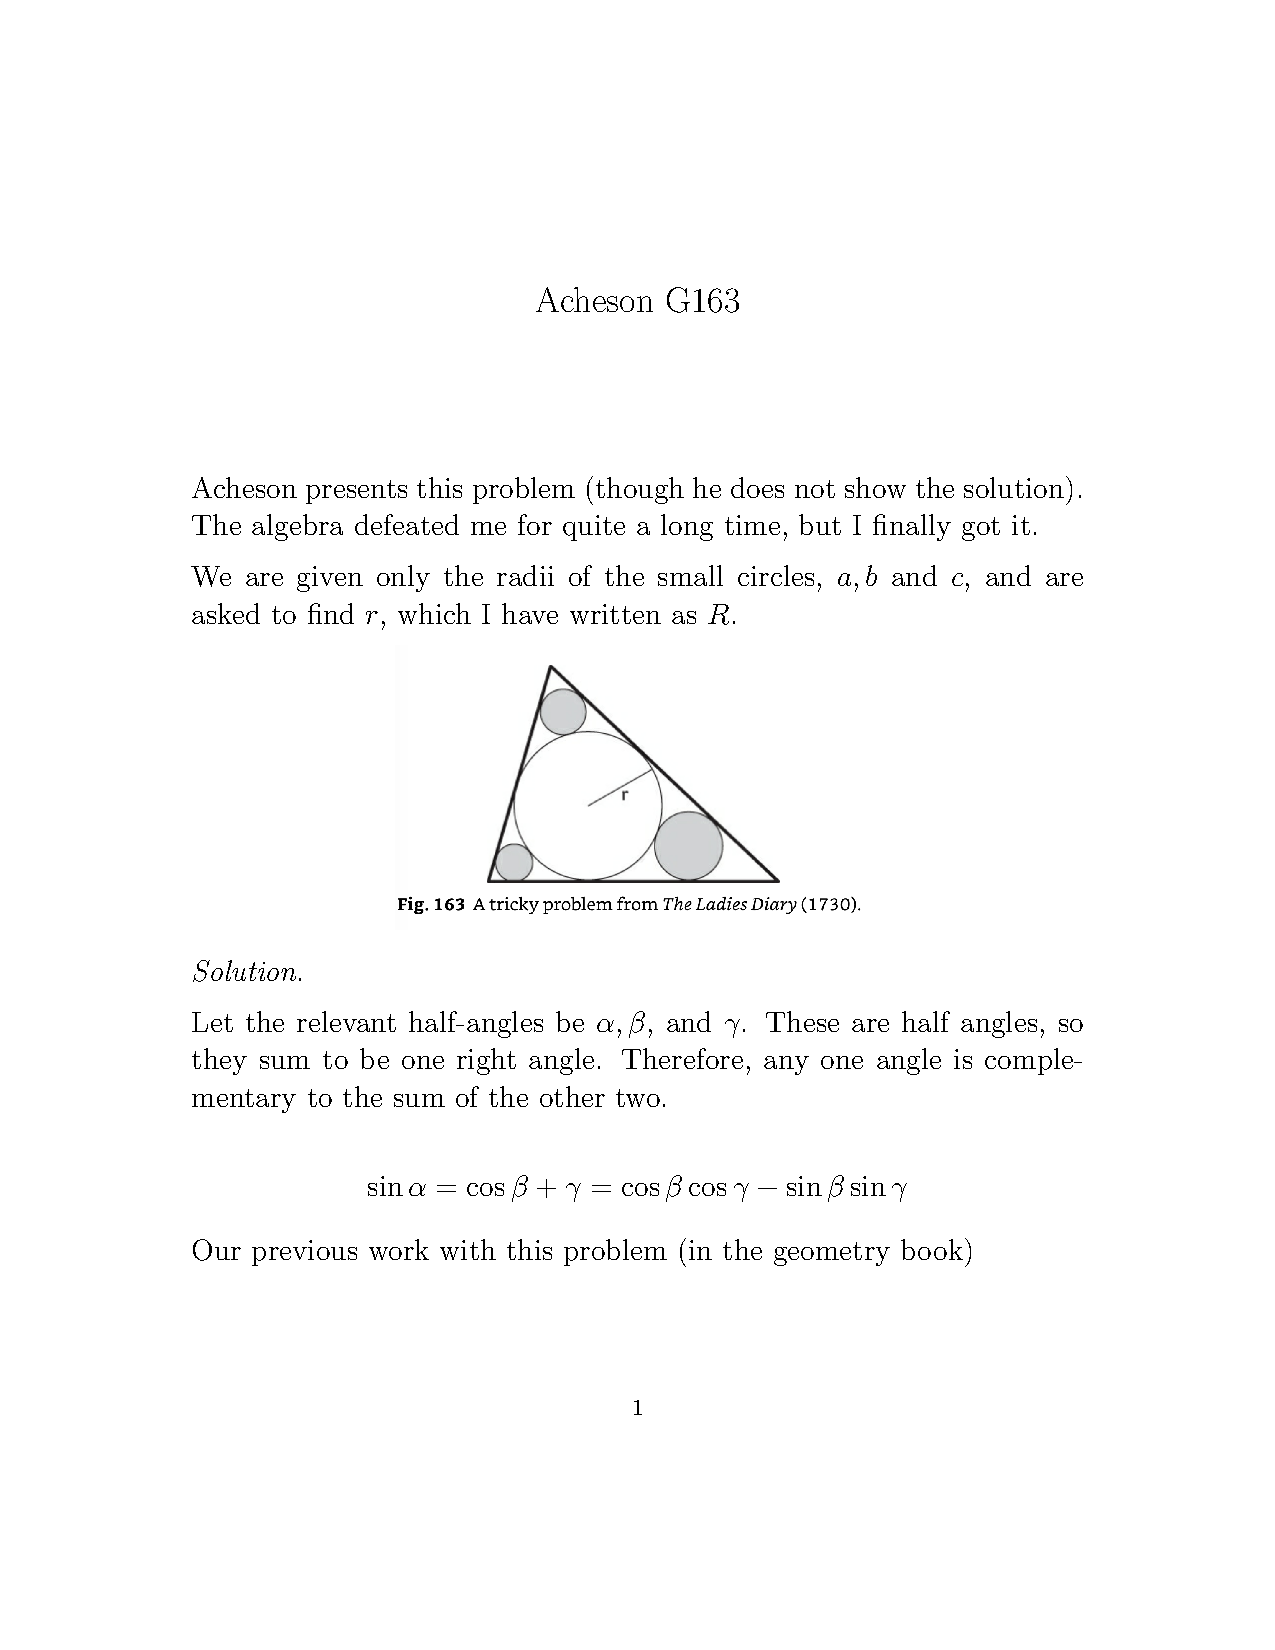
\includegraphics [scale=0.4] {Acheson_G163.png} \end{center}

\emph{Solution}.

Let the relevant half-angles at the vertices be $\alpha, \beta$, and $\gamma$.  These are half angles, so they sum to be one right angle.  Therefore, any one angle is complementary to the sum of the other two, and the sine of one is the cosine of the sum of the other two. 

\[ \sin \alpha = \cos \beta + \gamma = \cos \beta \cos \gamma - \sin \beta \sin \gamma \]

Our previous work with this problem (in the geometry book)
%\begin{center} \includegraphics [scale=0.5] {double_scoop1.png} \end{center}

showed that 
\[ \sin \theta = \frac{R - r}{R + r}, \ \ \ \ \ \ \cos \theta = \frac{2\sqrt{Rr}}{R + r} \]

Draw similar triangles involving the centers of the two circles to get this result.

We can apply this to the current problem, giving similar formulas for $\alpha$, $\beta$ and $\gamma$ in terms of the radii $a, b$ and $c$ as well as $R$.

So the expression for $\sin \alpha$ above can be written as 
\[ \frac{R - a}{R + a} = \frac{2\sqrt{Rb}}{R + b} \cdot \frac{2\sqrt{Rc}}{R + c} - \frac{R - b}{R + b} \cdot \frac{R - c}{R + c} \]

Rearranging:
\[ (R-a)(R+b)(R+c) + (R+a)(R-b)(R-c) = 4R \sqrt{bc} \cdot (R + a) \]

The first term is
\[ (R-a)(R+b)(R+c) \]
\[ = (R-a)(R^2 + Rb + Rc + bc) \]
\[ = R^3 + R^2b + R^2c + Rbc -R^2a - Rab - Rac - abc \]

The second term is 
\[ (R+a)(R-b)(R-c) \]
\[ = (R+a)(R^2 - Rb - Rc + bc) \]
\[ = R^3 - R^2b - R^2c + Rbc + R^2a - Rab - Rac + abc \]

The sum has four cancelations and four terms remaining:
\[ 2R^3 + 2Rbc - 2Rab - 2Rac =  4R \sqrt{bc} \cdot (R + a) \]

We can factor out $2R$
\[ R^2 + bc - ab - ac =  2 (R + a) \sqrt{bc} \]
\[ R^2 + bc - ab - ac =  2R \ \sqrt{bc} + 2a \sqrt{bc} \]

This is a quadratic in $R$:
\[ R^2 - 2 \sqrt{bc} \ R + bc - ab - ac - 2a \sqrt{bc} \]

The discriminant is
\[ 4bc - 4(bc - ab - ac - 2a \sqrt{bc}) \]

with another cancelation
\[ 4ab + 4ac + 8a \sqrt{bc} \]

The $4$ comes out from the square root as $2$ and we have
\[ R = \frac{2 \sqrt{bc} \pm 2 \sqrt{ab + ac + 2a \sqrt{bc}}}{2} \]
\[ R = \sqrt{bc} \pm \sqrt{ab + ac + 2a \sqrt{bc}} \]

But what is under the square root is a perfect square, namely
\[ ab + ac + 2a \sqrt{bc} = (\sqrt{ab} + \sqrt{ac})^2 \]

We have
\[ R = \sqrt{bc} \pm (\sqrt{ab} + \sqrt{ac}) \]

We will disregard the negative sign and obtain finally
\[ R = \sqrt{bc} + \sqrt{ab} + \sqrt{ac} \]

$\square$

As expected, it is symmetric in $a,b$ and $c$.


\end{document}